In this chapter we will first study the renormalisation group equations to understand how the couplings change with energy. This is achieved by first introducing the Callan-Symanzik equation \cite{Callan:1970yg, Symanzik:1970rt, Symanzik:1971vw}, followed by the computation of the non-Abelian gauge beta function. From this we will consider different scenarios of the coupling's behaviour when the energy scale is changed. Through this we introduce a core concept of the thesis: \textit{asymptotic freedom}.

\section{Renormalisation}
Quantum Field Theory (QFT) gives us the tools we need to understand the Universe's smallest structures. However, when applying this framework one encounters divergences when computing physical quantities. This raises a fundamental question: \textit{at what scale is the theory valid?} One framework to address this question is the renormalisation group (RG) \cite{Gell-Mann:1954yli}, particularly through \textit{Wilson}'s approach \cite{Wilson:1983xri, Wilson:1974mb}. The formalism provides a physical understanding of one of the key features of QFT, namely, renormalisation \cite{Pernow:2021fvb}.

These divergences arise when computing loop amplitudes, which must yield finite values to correspond to physical observables. The divergences are specifically encountered when integrating over internal momenta when computing Feynman diagrams \cite{Pernow:2021fvb}. To obtain finite amplitudes, one needs to first regularise the divergences. Methods of this include cutoff \cite{Peskin:1995ev}, Pauli-Villars \cite{Pauli:1949zm}, and dimensional regularisation \cite{tHooft:1972tcz}. All of these introduce an energy scale dependence, which we will call $\Lambda$, into the theory. We will see an example of this later in Section \ref{sec:betafunc}. 

The scale dependence introduced through the regularisation is not only a mathematical feature of the approach, but a physical attribute of the model. In Wilson's interpretation, the cutoff $\Lambda$ represents the energy scale at which the effective theory breaks down. The main effect of this approach is that masses and the coupling constants evolve as a function of $\Lambda$. An objective of this approach is therefore to extract how the coupling constants evolve with the energy scale. 

A theory will generally be described by a set of parameters $\{g_i\}$. These are mass parameters and couplings. If we wish to examine different length scales\footnote{Recall that using natural units where $c=\hbar=1$ the de Broglie wavelength is $p\propto1/\lambda$. In the relativistic limit this means that energy scales as one over length. So high energies is equal to short distances and vice versa. }, we can introduce a parameter $h$ to understand how the masses and couplings change with the energy scale at which we probe our theory
\begin{align} 
    g_i(\Lambda)\to g_i(\Lambda/h)\,,
\end{align}
where $h>1$ allows us to consider larger length scales, this is called \textit{coarse-graining} \cite{Lancaster:2014}. The variation of the parameter $h$ ensures rescaling of the cutoff $\Lambda$, and will therefore affect the values of the couplings. 

For a system with two couplings $g_i$ with $i=1,2$, the scale dependence can be visualised by multiple trajectories which change as the energy scale changes. These trajectories are called a renormalisation group trajectory and collection of these depict the renormalisation group flow \cite{Lancaster:2014}. An illustrated example can be found in Figure~\ref{fig:RGflow}. 
\begin{figure}[htbp]
    \centering
        \begin{tikzpicture}[
            scale=1.1,
            >={Stealth[scale=1.1]},
            flow/.style={
                thick,
                postaction={decorate}, 
                decoration={markings, mark=at position 0.55 with {\arrow{>}}}
            }
        ]

            % Axes
            \draw[->] (0,0) -- (3.5,0) node[right] {$g_1$};
            \draw[->] (0,0) -- (0,3.6) node[above] {$g_2$};

            % Top curve (Starts a bit further back, stays flat longer, curves up sharply)
            \filldraw (0.3, 2.6) circle (1.5pt);
            \draw[flow] (0.3, 2.6) .. controls (1.8, 2.6) and (2.5, 2.7) .. (3.2, 3.5);

            % Middle curve (Starts further forward, curves up gently and earlier)
            \filldraw (0.3, 1.7) circle (1.5pt);
            \draw[flow] (0.3, 1.7) .. controls (1.4, 1.7) and (2.2, 1.9) .. (3.0, 2.4);

            % Bottom curve (Starts in between, stays flat then drops off at the end)
            \filldraw (0.3, 0.9) circle (1.5pt);
            \draw[flow] (0.3, 0.9) .. controls (1, 0.9) and (2, 0.8) .. (2.9, 0.4);

        \end{tikzpicture}
        \vspace{0.5cm} % Alignment spacing
        \caption{Illustrative RG trajectories in the $(g_1,g_2)$ parameter space. The black dots mark the initial coupling values, with the arrows showing the RG flow, which point towards the UV.} 
        \label{fig:RGflow}
\end{figure}
% We can also consider the change of the coupling as In this space, \textit{fixed points} can occur. These are points in the multidimensional space defined by the set of couplings, which does not change with coarse-graining. \comment{insert sketch}

Now having reviewed the Wilsonian framework, we will follow the standard QFT approach of renormalising the Lagrangian. It is crucial here to distinguish the Wilsonian approach from the Callan--Symanzik approach (which we follow from now and in the following section). In Wilson's framework, the cutoff $\Lambda$ is a physical scale, and the RG flow describes how the effective theory changes as we integrate out physical high-energy modes. In contrast, the standard QFT approach aims to remove the cutoff entirely by taking the limit $\Lambda\to\infty$. To keep physical quantities finite, we absorb the divergences into counterterms, a process which inherently introduces a new, arbitrary energy scale called the renormalisation scale, $\mu$. Unlike Wilson's $\Lambda$, $\mu$ is strictly a mathematical artefact. Therefore in this approach, physical observables, such as the S-matrix, remain invariant under the change of the arbitrary energy scale $\mu$. 

We do this through renormalisation of the theory. Renormalisation ensures that the parameters of the Lagrangian change with the energy scale, effectively countering the effect of regularisation. Thus, the Lagrangian can be expressed as
\begin{equation}
    \mathcal{L}_{\mathrm{0}}= \mathcal{L}_{\mathrm{Renorm}}+ \mathcal{L}_{\mathrm{ct}}\label{eq:Barelag}
\end{equation} 
where $ \mathcal{L}_{\mathrm{0}}$ is the so-called \textit{bare} Lagrangian, which represent the theory's original Lagrangian containing the bare parameters which are the non-renormalised parameters. On the RHS $\mathcal{L}_{\mathrm{Renorm}}$ describes the renormalised Lagrangian, whose parameters are physical and depend on the energy scale,  and $ \mathcal{L}_{\mathrm{ct}}$ describes the necessary counterterms, which absorb the divergences. In this approach, we have already sent our cutoff to infinity, so how do we extract the RG flows of the parameters? We can use that the renormalisation of the Lagrangian depends on conditions at some renormalisation scale \cite{Peskin:1995ev}. Let us consider an example: a non-Abelian theory consisting of massless fermions. This theory has the bare Lagrangian
\begin{align}
    \mathcal{L}_0 = -\frac{1}{4} F^{a}_{0\mu\nu} F_0^{a\,\mu\nu}
+ \bar{\psi}_0 i \gamma^\mu D_\mu \psi_0\,,\label{eq:LagnonAbelian}
\end{align} 
with
\begin{equation}
D_\mu = \partial_\mu + i g_0 A^a_{0\mu} t^a\,, \qquad F^a_{\mu\nu}=\partial_\mu A_\nu^a-\partial_\nu A^a_\mu+g_0 f^{abc}A_\mu^bA_\nu^c\,,
\end{equation}
where \(g_0\) denotes the bare coupling constant, $\gamma^\mu$ are the Dirac matrices which obey the Clifford algebra, $f^{abc}$ is the structure constant of the concerned gauge group, and the gauge indices of the fermions have been suppressed for clarity. The bare parameters are related to the renormalised parameters as
\begin{equation}
\psi_0 = \sqrt{Z_2}\,\psi, \qquad
A^a_{0\mu} = \sqrt{Z_3}\,A^a_\mu, \qquad
g_0 = \mu^\epsilon Z_g\, g\,, \label{eq:Renormvalue}
\end{equation}
where $\mu^\epsilon$ is added to ensure a dimensionless coupling when using the dimensional regularisation scheme, which will be further explained in the subsequent section.
 
Now that we understand the motivation of the RG, we can use our knowledge to write down and equation which describes how the physical parameters of the theory will change with the energy scale, this is the \textit{Callan-Symanzik equation} \cite{Callan:1970yg,Symanzik:1970rt,Symanzik:1971vw}. 

\section{The Callan-Symanzik Equation}
In the process of dimensional regularisation the energy scale $\mu$ is introduced. This energy scale is not fixed and could just as well be given by $\mu'$. The only thing that needs to remain fixed is the bare Lagrangian $\mathcal{L}_{
\mathrm{0}}$ (see Eq.~\eqref{eq:Barelag}). 
Recall that the fields rescale as $\phi_0 = \sqrt{Z}\,\phi$ (see Eq.~\eqref{eq:Renormvalue}). This can be generalised for $n$ fields, so we can write the renormalised Green's function as a scaling of the bare Green's function
\begin{align}
    \langle \Omega | T\phi(x_1)\phi(x_2)\cdots\phi(x_n) |\Omega \rangle = Z^{-n/2} \langle \Omega | T\phi_0(x_1)\phi_0(x_2)\cdots\phi_0(x_n) |\Omega \rangle\,.
\end{align}
The bare Lagrangian will, by definition, remain scale invariant, since it is describing the underlying theory. Scale-dependency emerges in the renormalised Lagrangian, because it is introduced to remove the cutoff-dependent $\lambda_0$ with a running coupling $\lambda$. As already pointed out, this scale could be chosen as $\mu'$ by mapping $\lambda\to\lambda'$ and $Z\to Z'$ \cite{Peskin:1995ev}. We can perform this shift $\delta\mu$ explicitly, which results in
\begin{align}
    \mu\to \mu+\delta \mu\,,\\\lambda\to\lambda+\delta\lambda\,,\\Z\to Z+\delta Z\,.
\end{align}
The shift of the Green's function is thus only dependent on the shift of the renormalisation constant $Z$
\begin{align}
    G^{(n)}\to G^{(n)}+\delta G^{(n)} = \left(Z^{-n/2}+\delta\left(Z^{-n/2}\right)\right) G_0^{(n)}\,,
\end{align}
where $G^{(n)}(x_1,\dots,x_n)=\langle \Omega | T\phi(x_1)\phi(x_2)\cdots\phi(x_n) |\Omega \rangle $. We can expand the second term
\begin{align}
    \left(\delta\left(Z^{-n/2}\right)\right)= \frac{ \partial \left(Z^{-n/2}\right)}{\partial Z}\delta Z=-\frac{n}{2} Z^{-n/2}\frac{\delta Z}{Z}= n \delta \eta\,, \label{eq:defeta}
\end{align}  
where $\delta\eta:=-\frac{1}{2}\frac{\delta Z}{Z}$. Thus, the shift in a renormalised Green's function is a field scaling 
\begin{align}
    G^{(n)}\to (1+n\delta\eta ) G^{(n)}\,.
\end{align}
We can now use the fact that the $n$-point Green's function $G^{(n)}$ is not only a function of spacetime but also the renormalisation scale and the renormalised coupling. $G^{(n)}(x_1,\dots,x_n;\mu,\lambda)$. Thus, the shift can be rewritten as
\begin{align}
    \delta G^{(n)} = \frac{\partial G^{(n)}}{\partial \mu} \delta \mu + \frac{\partial G^{(n)}}{\partial \lambda} \delta \lambda\,.
\end{align}
We can use the definition from Eq.~\eqref{eq:defeta} to obtain 
\begin{align}
     \left[\frac{\partial}{\partial \mu} \delta \mu + \frac{\partial}{\partial \lambda} \delta \lambda- n\delta\eta \right]G^{(n)}(x_1,\dots,x_n;\mu,\lambda)=0\,,\label{eq:CSeq1}
\end{align}
and by defining 
\begin{align}
    \beta\equiv \frac{\mu}{\delta\mu}\delta\lambda\,, \qquad  \gamma\equiv- \frac{\mu}{\delta\mu}\delta\eta\,,\label{eq:beta0}
\end{align}
the expression in Eq.~\eqref{eq:CSeq1} can be rewritten as 
\begin{align}
     \left[\mu\frac{\partial}{\partial \mu}  + \beta \frac{\partial}{\partial \lambda} + n\gamma \right]G^{(n)}(x_1,\dots,x_n;\mu,\lambda)=0\,.
\end{align}
It is of importance to understand what the parameters $\beta$ and $\gamma$ depend on. First, they cannot depend on $n$ since the expression holds for all $n-point$ functions. Furthermore, they are independent of $x_i$, since the parameters are properties of the theory itself and not kinematic effects. Because the Green's function is renormalised, they cannot depend on the cutoff $\Lambda$. Additionally, the parameters cannot depend explicitly on the energy scale; this can be seen by the fact that both parameters are dimensionless, and the energy scale is not. The only dependency of the parameters are thus the couplings, so we can write 
\begin{align}
     \left[\mu\frac{\partial}{\partial \mu}  + \beta(\lambda) \frac{\partial}{\partial \lambda} + n\gamma(\lambda) \right]G^{(n)}(\{x_i\};\mu,\lambda)=0\,.
\end{align}
This is the Callan--Symanzik equation, which describes how the change of the scale at which we are probing our theory is balanced by changes to the two parameters $\beta$ and $\gamma$. The case above is only for a theory with one massless field and one coupling. An additional coupling translates to an additional $\beta$ parameter, and an additional field ensures that there will be an extra $\gamma$ parameter. Furthermore, it should be noted that this analysis changes when considering a massive theory. Since the mass is also renormalised, the Green's function will also depend on the mass, which runs with the energy scale $\mu$. The general Callan--Symanzik equation is then expressed as \cite{Srednicki2007}
\begin{align}
     \left[\mu\frac{\partial}{\partial \mu}  + \beta(\lambda) \frac{\partial}{\partial \lambda} +\gamma_m\frac{\partial }{\partial \ln m}+ n\gamma(\lambda) \right]G^{(n)}(\{x_i\};\mu,\lambda, m)=0\,,
\end{align}
where $\gamma_m=\frac{\partial \ln m}{\partial \ln \mu}$ is called the \textit{anomalous dimension of the mass} and describes how changing the energy scale affects the renormalised mass \cite{Srednicki2007}. 

With the RG framework established, we shift our focus to the introduced parameter $\beta$. The subsequent section provides a deeper insight into the mechanics of the beta function by considering an example. Through this example we will apply the mathematical tools we have already discussed: first regularisation and then renormalisation. This approach also allows us to understand how the couplings can run.

\section{The beta function} \label{sec:betafunc}
To better understand the new parameters $\beta$ and $\gamma$, we can consider the limit in which $\delta\to\partial$ of Eq.~\eqref{eq:beta0}, from which we obtain
\begin{align}
    \beta\equiv \mu\frac{\partial \lambda}{\partial\mu}\,, \qquad  \gamma\equiv- \mu\frac{\partial\eta}{\partial\mu}=-\frac{\mu}{Z}\frac{\partial Z}{\partial \mu}\,.\label{eq:betafunc}
\end{align}
The parameters are referred to as the \textit{beta function} and \textit{anomalous dimension} \cite{Pernow:2021fvb}. As seen from the formula and explained above, the equation shows the coupling's and the field's reaction to the change of the energy scale, respectively. Our interest lies predominantly in the beta function, because this describes the change of the interaction strength between our fields as the energy scale at which we probe our theory changes. The approach to calculating these Callan--Symanzik functions is through the counterterms originating from the renormalisation. We can relate the beta function directly to these.

\subsection{An example: Non-Abelian Lagrangian}
Let us take the example of the bare Lagrangian $\mathcal{L}_\mathrm{0}$ in Eq.~\eqref{eq:LagnonAbelian} describing non-Abelian gauge theories with massless fermions. To generalise the beta function we will extend the theory to include massive fermionic fields effectively adding a term to the bare Lagrangian, so that the full Lagrangian yields \cite{Peskin:1995ev}
\begin{align}
     \mathcal{L}_\mathrm{0} &= \bar{\psi}(i \slashed{\partial} - m)\psi - \frac{1}{4}(\partial_\mu A_\nu^a - \partial_\nu A_\mu^a)^2 + g_0 A_\mu^a \bar{\psi} \gamma^\mu t^a \psi\nonumber \\&\quad- g_0 f^{abc} (\partial_\mu A_\nu^a) A^{\mu b} A^{\nu c} - \frac{1}{4} g_0^2 (f^{eab} A_\mu^a A_\nu^b)(f^{ecd} A^{\mu c} A^{\nu d})\,.\label{eq:LnonA}
\end{align}
In the Lagrangian the third term is the vertex, which we can write in its renormalised form as
\begin{equation}
    \Gamma_{\bar{\psi} A \psi, r}^{(3)} = \Gamma_{\bar{\psi} A \psi}^{(3)} / Z_1 \,.
\end{equation}
Thus, we can express the renormalised coupling using Eq.~\eqref{eq:Renormvalue} as 
\begin{align}
    Z_1 g_r =\mu^{-\epsilon} \sqrt{Z_2} \sqrt{Z_3} \sqrt{Z_2} g_0 = \mu^{-\epsilon} Z_2 Z_3^{1/2} g_0 \implies g_r = \mu^{-\epsilon}\frac{Z_2 Z_3^{1/2}}{Z_1} g_0 \,,
\end{align}
where $g_r$ is the fermion-gauge coupling. We can then consider the beta function (see Eq.~\eqref{eq:betafunc}) of the coupling
\begin{equation}
    \beta(g_r) = \mu \frac{\dd g_r}{\dd\mu}\,.
\end{equation}
From now on, we will drop the subscript on the coupling and set $g_r = g$. We have
\begin{align}
    \beta(g)  &= \mu \frac{\partial}{\partial\mu} \left(\mu^{-\epsilon} \frac{Z_2 Z_3^{1/2}}{Z_1} g_0 \right)\nonumber \\
    &=-\epsilon g +g_0 \left( \frac{Z_2 Z_3^{1/2}}{Z_1} \mu \frac{\partial}{\partial\mu} \ln\left( \frac{Z_2 Z_3^{1/2}}{Z_1} \right) \right) \nonumber\\
    &= -\epsilon g+g \left( \mu \frac{1}{Z_2} \frac{\partial Z_2}{\partial\mu} + \frac{\mu}{2 Z_3} \frac{\partial Z_3}{\partial\mu} - \frac{\mu}{Z_1} \frac{\partial Z_1}{\partial\mu} \right)\,,
\end{align}
where we used that the derivative of the bare coupling is zero $\frac{\partial}{\partial\mu} g_0 = 0$, since the bare parameters, by definition, do not change with the energy scale. 

We can now use the definition of the anomalous dimensions in Eq.~\eqref{eq:betafunc} to identify
\begin{equation}
    \gamma_i = - \frac{\mu}{Z_1}  \frac{\partial Z_i}{\partial\mu} \sim -\mu  \frac{\partial \delta_i}{\partial \mu}\,,
\end{equation}
where we use that $Z_i=1+\delta_i$ where $1$ is the three level contribution and $\delta_i$ the counterterm, and $\delta_i\ll 1$. This allows us to approximate the beta function as
\begin{align}
    \beta(g) =-\epsilon g+ g  \frac{\partial}{\partial\mu} \left( \gamma_1 - \gamma_2 - \frac{1}{2} \gamma_3 \right) \sim-\epsilon g+ g \mu \frac{\partial}{\partial\mu} \left( -\delta_1 + \delta_2 + \frac{1}{2} \delta_3 \right) \,.
\end{align}
Thus, the process of calculating a beta function boils down to computing counterterms and thereby Feynman loop diagrams. In general, we distinguish between the loop order of the beta function. Let us compute the example we have been considering so far: the one-loop gauge beta function of the non-Abelian theory with one massive fermionic field. 

We will only do one of the calculations here explicitly, as this provides a clear example of how to perform such calculations. The different contributions come from the one-loop diagrams of  the fermion-gauge boson vertex
\begin{align}\delta_1\sim \raisebox{-0.8cm}{\feynmandiagram [vertical=a to b, small] {
        a -- [photon] b ,
        f1 -- [fermion] c -- [fermion] b -- [anti fermion] d -- [fermion] f2,
        c -- [photon] d,
    };}+\raisebox{-0.8cm}{\feynmandiagram [vertical=a to b, small] {
        a -- [photon] b ,
        f1 -- [fermion] c -- [photon] b -- [photon] d -- [fermion] f2,
        c -- [fermion] d,
    };}\,,\label{eq:delta1}
\end{align}
the fermion self-energy
\begin{align}
    % Electron Self-Energy
    \delta_2 &\sim \raisebox{-0.1cm}{
        \begin{tikzpicture}
            \begin{feynman}
                \vertex (a);
                \vertex [right=1cm of a] (c);
                \vertex [right=1.5cm of c] (d);
                \vertex [right=1cm of d] (b);
                \diagram* {
                    (a) -- [plain] (c) -- [fermion] (d) -- [plain] (b),
                    (c) -- [photon, half left, looseness=1.5] (d),
                };
            \end{feynman}
        \end{tikzpicture}
    } \,,\label{eq:delta2}
\end{align}
and the gauge boson self-energy 
\begin{align}
    % Vacuum Polarisation (Fermion Loop)
    \delta_3 \sim \raisebox{-0.6cm}{
        \begin{tikzpicture}
            \begin{feynman}
                \vertex (a);
                \vertex [right=0.8cm of a] (c);
                \vertex [right=1.2cm of c] (d);
                \vertex [right=0.8cm of d] (b);
                \diagram* {
                    (a) -- [photon] (c),
                    (c) -- [fermion, half left, looseness=1.5] (d) -- [fermion, half left, looseness=1.5] (c),
                    (d) -- [photon] (b),
                };
            \end{feynman}
        \end{tikzpicture}
    } + \raisebox{-0.6cm}{
        % Boson/Gauge Loop
        \begin{tikzpicture}
            \begin{feynman}
                \vertex (a);
                \vertex [right=0.8cm of a] (c);
                \vertex [right=1.2cm of c] (d);
                \vertex [right=0.8cm of d] (b);
                \diagram* {
                    (a) -- [photon] (c),
                    (c) -- [photon, half left, looseness=1.5] (d) -- [photon, half left, looseness=1.5] (c),
                    (d) -- [photon] (b),
                };
            \end{feynman}
        \end{tikzpicture}
    }  + \raisebox{-0.6cm}{
        % Scalar Loop
        \begin{tikzpicture}
            \begin{feynman}
                \vertex (a);
                \vertex [right=0.8cm of a] (c);
                \vertex [right=1.2cm of c] (d);
                \vertex [right=0.8cm of d] (b);
                \diagram* {
                    (a) -- [photon] (c),
                    (c) -- [scalar, half left, looseness=1.5] (d) -- [scalar, half left, looseness=1.5] (c),
                    (d) -- [photon] (b),
                };
            \end{feynman}
        \end{tikzpicture}
    } + \raisebox{-0.3cm}{ 
        % Adjusted raisebox because legs are lower now
        \begin{tikzpicture}
            \begin{feynman}
                % Angled legs: start below the interaction vertex
                \vertex (a) at (0, -0.3); 
                \vertex (c) [dot] at (1.0, 0); % The centre
                \vertex (b) at (2.0, -0.3);
                % The loop anchor
                \vertex (d) at (1.0, 0.8); 
                \diagram* {
                    (a) -- [photon] (c) -- [photon] (b),
                    (c) -- [photon, half left, looseness=1.6] (d) -- [photon, half left, looseness=1.6] (c),
                };
            \end{feynman}
        \end{tikzpicture}
    }\,.\label{eq:delta3}
\end{align}
The diagrams in Eq.~\eqref{eq:delta1} represent the vertex renormalisation. The first diagram is also present in the vertex corrections of Abelian theories. The second diagram is specific to non-Abelian theories, since it includes self-interactions between the gauge bosons. Thus, $\delta_1$ will absorb the divergences of these two one-loop diagrams. In Eq.~\eqref{eq:delta2} $\delta_2$ is defined to renormalise the fermion wave function. Lastly, Eq.~\eqref{eq:delta3} represents the gauge boson wave function corrections, coming from four one-loop diagrams, including a fermion loop, a ghost loop,\footnote{Faddeev--Popov ghosts are unphysical fields and are introduced to combat gauge redundancy \cite{Peskin:1995ev}.} and two including gauge boson self-interactions. The last diagram is generally called a tadpole diagram.\footnote{This diagram can equal zero depending on the chosen regularisation scheme \cite{Peskin:1995ev}.}

We choose to focus on the contributions from the fermion self-energy, $\delta_2$ in Eq.~\eqref{eq:delta2}. The other terms are given by \cite{Peskin:1995ev}
\begin{align}
   \delta_1 &= -\frac{g^2}{(4\pi)^{d/2}} \frac{\Gamma(2 - d/2)}{(\mu^2)^{2-d/2}} [C_2(R) + C_2(G)] \,,\label{eq:delta1expr}\\
   \delta_3& =\frac{g^2}{(4\pi)^{d/2}} \frac{\Gamma(2 - d/2)}{(\mu^2)^{2-d/2}} \left[ \frac{5}{3} C_2(G) - \frac{4}{3} n_f T(R) \right]\,,\label{eq:delta3expr} 
\end{align}
where $n_f$ is the number of different fermion fields. There are three group-theoretical (see Appendix \ref{app:GT}) constants in the equations, two of them depend on the gauge group and the representation $R$ of the fermionic field(s): $T(R)$ is the Dynkin index and $C_2(R)$ is the quadratic Casimir index. The factor $C_2(G)$ is the quadratic Casimir as well, but of the gauge group $G$ (see Appendix~\ref{app:Lie}).

To compute the renormalised fermion's self-energy \(-i \Sigma_R(p^2)\), we need to include the counterterm contributions. These terms absorb the UV divergences of the loop diagrams, rendering the physical quantity finite through a proper choice of  $\delta_2$ and $\delta_m$. Thus, we need to calculate the sum of the two diagrams, the loop diagram and the corresponding counterterm, given by 
\begin{align}
     -i \Sigma_{\mathrm{R}}(p^2)=-i \Sigma_{\text{1 loop}}(p^2)+i(\slashed{p}\delta_2-\delta_m)= \raisebox{-0.1cm}{
        \begin{tikzpicture}
            \begin{feynman}
                \vertex (a);
                \vertex [right=1cm of a] (c);
                \vertex [right=1.5cm of c] (d);
                \vertex [right=1cm of d] (b);
                \diagram* {
                    (a) -- [plain] (c) -- [fermion] (d) -- [plain] (b),
                    (c) -- [photon, half left, looseness=1.5] (d),
                };
            \end{feynman}
        \end{tikzpicture}
    } 
    + 
    \raisebox{-0.1cm}{
        \begin{tikzpicture}
            \begin{feynman}
                \vertex (a) at (0, 0); 
                \node [draw, circle, minimum size=10pt, inner sep=0pt] (c) at (1.2, 0) {};
                \vertex (b) at (2.4, 0);
                % Draw the cross manually
                \draw (c.north west) -- (c.south east);
                \draw (c.north east) -- (c.south west);
                \diagram* {
                    (a) -- [plain] (c) -- [plain] (b),
                };
            \end{feynman}
        \end{tikzpicture}
    }\,,\label{eq:fermselfenergy}
\end{align}
where the structure of the counterterm originates for the kinetic term of fermion in the Lagrangian in Eq.~\eqref{eq:LnonA}. To compute the one-loop diagram, we need the three following Feynman rules \cite{Peskin:1995ev}:
\begin{align}
  &\text{Vertex: } ig \gamma^\mu t^a\label{eq:fey1}\,,\\
  &\text{fermion propagator: } \frac{i(\slashed{p} + m)}{p^2 - m^2 + i \epsilon}\,, \\
  &\text{boson propagator:} -\frac{i g_{\mu\nu}}{q^2 + i \epsilon}\label{eq:fey3}\,,
\end{align}
where the boson propagator is found using the Feynman-'t Hooft gauge.


The diagram has an incoming fermion momentum \(p\), an internal fermion momentum \(k\), and an internal boson momentum \(p-k\). We can use this together with the Feynman rules (Eqs. \eqref{eq:fey1}-\eqref{eq:fey3}) to write
\begin{align}
  -i \Sigma_{\text{1 loop}}(p^2) &=\raisebox{-0.7cm}{
    \begin{tikzpicture}
        \begin{feynman}
            \vertex (a);
            \vertex [right=1cm of a] (c);
            \vertex [right=1.5cm of c] (d);
            \vertex [right=1cm of d] (b);
            \diagram* {
                (a) -- [fermion, momentum=\(p\)] (c) -- [fermion, momentum'=\(k\)] (d) -- [fermion, momentum=\(p\)] (b),
                (c) -- [photon, half left, looseness=1.5, momentum=\(p-k\)] (d),
            };
        \end{feynman}
    \end{tikzpicture}
}\nonumber\\&= \int \frac{\dd^4 k}{(2\pi)^4} ig \gamma^\mu t^a \frac{i(\slashed{k} + m)}{k^2 - m^2 + i \epsilon} ig \gamma^\nu t^a \frac{-i g_{\mu\nu}}{(p-k)^2 + i \epsilon}\nonumber\\
  &= -g^2\int \frac{\dd^4 k}{(2\pi)^4} \gamma^\mu t^a \frac{\slashed{k} + m}{k^2 - m^2 + i \epsilon} \gamma_\mu t^a \frac{1}{(p-k)^2 + i \epsilon}\,.
\end{align}
We can now use the group theory relation of the operators \(t^a t^a = C_2(R) \mathbb{1}\) (see Appendix \ref{app:Lie}) to simplify the expression, such that we obtain
\begin{align}
  -i \Sigma_{\text{1 loop}}(p^2)&= -g^2 C_2(R) \int \frac{\dd^4 k}{(2\pi)^4} \gamma^\mu \frac{\slashed{k} + m}{k^2 - m^2 + i \epsilon} \gamma_\mu \frac{1}{(p-k)^2 + i \epsilon}\,.
\end{align}
To simplify the numerator we use the relations $\gamma^\mu\gamma_\mu=d\mathbb{1}$ and $\gamma^\mu\gamma_\mu\gamma^\nu=(2-d)\gamma^\nu$ \cite{Peskin:1995ev}, which yields
\begin{align}
   \gamma^\mu(\slashed{k}+m)\gamma_\mu&=\gamma^\mu\gamma^\nu k_\nu\gamma_\mu+\gamma^\mu m\gamma_\mu=k_\nu\gamma^\mu\gamma^\nu\gamma_\mu+md\mathbb{1}=k_\nu(2-d)\gamma^\nu+md=-((d-2)\slashed{k} - md)\,.
\end{align}
This results in the following integral
\begin{align}
  -i \Sigma_{\text{1 loop}}(p^2) = g^2 C_2(R) \int \frac{\dd^4 k}{(2\pi)^4} \frac{(d-2)\slashed{k} - md}{(k^2 - m^2 + i\epsilon)((p-k)^2 + i\epsilon)} \,.\label{eq:den}
\end{align}
The next step is to use Feynman parameterisation. Utilising this method we can transform the two factors in the denominator in Eq.~\eqref{eq:den} into a single quadratic polynomial in $k$. This polynomial will be squared. Then we can shift the integration momentum $k$ to complete the square leaving us with a spherically symmetric denominator. The price to pay for this is an additional integral over a Feynman parameter. We can write this as
\begin{align}
    \frac{1}{AB} = \int_0^1 \frac{\dd x}{[(1-x)A + xB]^2}\,.\label{eq:Feypar}
\end{align}
To use this method, we first define $A$ and $B$ by considering the denominator in Eq.~\eqref{eq:den}. Then we can expand the expression of the denominator, which yields
\begin{align}
    A &= k^2 - m^2 + i\epsilon \,,\\
    B &= (p-k)^2 + i\epsilon = p^2 + k^2 - 2pk + i\epsilon \,,\\
    D &= (1-x)(k^2 - m^2 + i\epsilon) + x(p^2 + k^2 - 2pk + i\epsilon)\nonumber\\
    &= k^2 - (1-x)m^2 + i\epsilon - i\epsilon x - k^2 x + xp^2 + x k^2 - 2pkx + i\epsilon x \nonumber\\
    &= k^2 + xp^2 - 2pkx - (1-x)m^2 + i\epsilon\,.
\end{align}
We can then complete the square by adding and subtracting $x^2p^2$, allowing us to obtain
\begin{align}
    D&= (k - xp)^2 - x^2p^2 + xp^2 - (1-x)m^2 + i\epsilon \nonumber\\
    &= \ell^2 + x(1-x)p^2 - (1-x)m^2 + i\epsilon \nonumber\\
    &= \ell^2 - \Delta + i\epsilon\,,\label{eq:denny}
\end{align}
with $\Delta = -x(1-x)p^2 + (1-x)m^2$ and $ \ell = k - xp$. Next, the numerator in Eq.~\eqref{eq:den} is rewritten in terms of the new variables, from which we obtain
\begin{align}
    N &= (d-2)\slashed{k} - dm \implies N=(d-2)(\slashed{\ell} + x\slashed{p}) - dm\,.\label{eq:numny}
\end{align}
We can now insert the redefinition of the numerator (Eq.~\eqref{eq:numny}) and the denominator (Eq.~\eqref{eq:denny}) using the Feynman parametrisation (Eq.~\eqref{eq:Feypar}) on our integral in Eq.~\eqref{eq:den}. Then we perform a Wick rotation to perform a spherical integral in four-dimensions. We do this by rotating the temporal component of the momentum four-vector $\ell_E = -i \ell^0$. This effectively transforms Minkowski space into a four-dimensional Euclidean space. This changes our momentum related terms to: 
\begin{align}
    &\dd^4\ell = \dd\ell_0 d^3\vec{\ell} \implies i \dd\ell_E^0 \dd^3\vec{\ell}_E = i \dd^4\ell_E\,,\\
    &\ell^2 - \Delta \implies -\ell_E^2 - \Delta = -(\ell_E^2 + \Delta) \,,
\end{align}
where we have dropped the $i\epsilon$ term, since in Euclidean space the denominator no longer vanishes for on shell particles. This leaves us with the Wick rotated integral
\begin{align}
    -i \Sigma_{\text{1 loop}}(p^2)= g^2 C_2 \int_0^1 \dd x \int \frac{\dd^4(i\ell_E)}{(2\pi)^4} \frac{(d-2)(x\slashed{p}) - dm}{[\ell_E^2 + \Delta]^2}\,,\label{eq:nyint}
\end{align}
where the terms linear in $\slashed{\ell}$ vanish since it is an odd function evaluated over a symmetric interval. To solve the integral, we can use the general relation \cite{Peskin:1995ev} given by
\begin{align}
    \int \frac{\dd^d \ell_E}{(2\pi)^d} \frac{1}{[\ell_E^2 + \Delta]^n} &= \Delta^{-n} \left(\frac{\Delta}{4\pi}\right)^{d/2} \frac{\Gamma(n - \frac{d}{2})}{\Gamma(n)}\,.
\end{align}
This relation can solve the integral over $\ell$ (Eq.~\eqref{eq:nyint}), leaving us with
\begin{align}
    -i \Sigma_{\text{1 loop}}(p^2)= i g^2 C_2 \frac{\Gamma(2 - \frac{d}{2})}{(4\pi)^{d/2}} \int_0^1 \dd x \left( (2-d)x\slashed{p} - dm \right) \Delta^{d/2 - 2}\,,\label{eq:int3}
\end{align}
where it has been used that  $\Gamma(2) = 1$ \cite{Peskin:1995ev}. The next step is to impose the renormalisation condition\footnote{This condition comes from the requirement that the pole in the two-point-function have a residue of one. We impose this condition at the arbitrary scale $\mu$.}
\begin{align}
    \frac{\dd}{\dd\slashed{p}} \left[ -i \Sigma_{\text{1loop}} (p^2) \Big|_{p^2=0, m=\mu} \right] &= 0\,.\label{eq:con}
\end{align}
Recall that the complete expression of the fermion self-energy is given by 
\begin{align}
    -i \Sigma_{\text{R}}(p^2)=-i \Sigma_{\text{1 loop}}(p^2)+i(\slashed{p}\delta_2-\delta_m)\,,
\end{align}
which we can differentiate with respect to $\slashed{p}$
\begin{align}
    \frac{\dd}{\dd\slashed{p}} (-i \Sigma) &= \frac{\dd}{\dd\slashed{p}} (-i \Sigma^{(1)}) + i \delta_2\,.
\end{align}
The condition on the fermion self-energy is found by inserting our integral Eq.~\eqref{eq:int3} and differentiating, which results in
\begin{align}
    0 &= i g^2 C_2 \frac{\Gamma(2 - \frac{d}{2})}{(4\pi)^{d/2}} (2-d) \int_0^1 dx \frac{x}{\Delta^{2 - d/2}} + i \delta_2\,,
\end{align}
where the derivative removes the dependence on the mass since the $dm$ term does not depend on $\slashed{p}$. The condition (see Eq. \eqref{eq:con}) also fixes the momentum and mass to $p^2 = 0$ and $m=\mu$, which allows us to simplify the expression of $\delta_2$, as follows
\begin{align}
    \delta_2 &= -g^2 C_2 \frac{\Gamma(2 - \frac{d}{2})}{(4\pi)^{d/2}} (2-d) \int_0^1 dx \frac{x}{((1-x)\mu^2)^{2 - d/2}} \nonumber\\
    &= g^2 C_2 \frac{\Gamma(2 - \frac{d}{2})}{(4\pi)^{d/2}} \frac{1}{(\mu^2)^{2 - d/2}} \underbrace{(d-2)\int_0^1 dx \frac{x}{(1-x)^{2 - d/2}}}_{K}\,,\label{eq:delta2expr}
\end{align}
where we refrain of simplifying $K$ for now. To obtain the beta function, we need to add all the contributions together using Eq.~\eqref{eq:delta1expr}, \eqref{eq:delta2expr}, and \eqref{eq:delta3expr}, we obtain 
\begin{align}
    -\delta_1 + \delta_2 + \frac{1}{2} \delta_3 &= \frac{g^2}{(4\pi)^{d/2}} \frac{\Gamma(2 - \frac{d}{2})}{(\mu^2)^{2-d/2}} \left[ C_2(R) + C_2(G) + \frac{5}{6} C_2(G) - \frac{4}{6} n_f T(R) + K C_2(R) \right] \\
    &= \frac{g^2}{(4\pi)^{d/2}} \frac{\Gamma(2 - \frac{d}{2})}{(\mu^2)^{2 - d/2}} \left[ C_2(R)(1 + K) + \frac{11}{6} C_2(G) - \frac{2}{3} n_f T(R) \right]\,.\label{eq:d123}
\end{align}
The next step is to regularise the expression. This is done using dimensional regularisation (unlike cutoff regularisation this method does not break gauge invariance \cite{Peskin:1995ev}). This method considers a variable spacetime dimensions and introduces a parameter $\epsilon$ such that $d=4-\epsilon$. Then we take the limit of $\epsilon\to0$ to recover our four dimensional world \cite{tHooft:1972tcz}.

First, we replace $d$ in Eq, \eqref{eq:d123}, which yields
\begin{align}
    -\delta_1+\delta_2+\frac{1}{2}\delta_3=\frac{g^2}{(4\pi)^{2}} \left(\frac{4 \pi}{\mu^{2}} \right)^{\epsilon/2}\Gamma\left(\frac{\epsilon}{2}\right)\left[ C_2(R)(1 + K) + \frac{11}{6} C_2(G) - \frac{2}{3} n_f T(R) \right]\,.
\end{align}
If we now insert this in the expression of the beta function, we have to differentiate the sum with respect to the energy scale, from which we obtain
\begin{align}
    \beta(g)&=\frac{g^3}{16\pi^2} \left( \frac{2}{\epsilon} + \mathcal{O}(\epsilon^0) \right) (4\pi)^{\epsilon/2} \mu (-\epsilon) \frac{1}{\mu^{\epsilon+1}} \left[ C_2(R)(1 + K) + \frac{11}{6} C_2(G) - \frac{2}{3} n_f C(R) \right]\nonumber\\
    &= \frac{-2g^3}{16\pi^2} \left( \frac{4\pi}{\mu^2} \right)^{\epsilon/2} \left[ C_2(R)(1 + K) + \frac{11}{6} C_2(G) - \frac{2}{3} n_f T(R) \right] + \mathcal{O}(\epsilon^0)\,.\label{eq:withoutK}
\end{align}
The remaining integral $K$ can be computed by utilising dimensional regularisation and taking the limit $\epsilon\to0$, we find
\begin{align}
    K &= (2-(4-\epsilon)) \int_0^1 \dd x \frac{x}{(1-x)^{\epsilon/2}} \nonumber\\
    &= (-2+\epsilon) \int_0^1 \dd x \frac{x}{(1-x)^{\epsilon/2}}\nonumber \\
    &= -2 \int_0^1 dx\ x + \mathcal{O}(\epsilon) \nonumber\\
    &= -2 \left[ \frac{1}{2} x^2 \right]_0^1 = -1\,,
\end{align}
where we have used the expansion of the denominator to lowest order in  $\epsilon$
\begin{align}
    (1-x)^{-\epsilon/2} = \exp[-\frac{\epsilon}{2} \ln(1-x)] \sim 1 +\frac{\epsilon}{2}\ln(1-x) + \mathcal{O}(\epsilon^2)\,.
\end{align}    
Inserting this back into Eq.~\eqref{eq:withoutK} and recalling the limit of $\epsilon\to0$, we obtain
\begin{align}
    \beta(g)&= \lim_{\epsilon\to0}\frac{-2g^3}{16\pi^2} \left( \frac{4\pi}{\mu^2} \right)^{\epsilon/2}\left[ C_2(R) (1 + (-1)) + \frac{11}{6} C_2(G) - \frac{2}{3} n_f C(R) \right] \nonumber\\&=
     \frac{-g^3}{16\pi^2} \left[ \frac{11}{3} C_2(G) - \frac{4}{3} n_f C(R) \right]\label{eq:derivedbetag}
\end{align}
where for $\SU(N)$ these values are given by $C_2(H) = N$, $T(R) = 1/2$ (see Appendix \ref{app:GT}). 

The general one-loop gauge beta function \cite{Gross:1973ju}, when including scalars as well as fermions, is given by
\begin{equation}
    \beta(\alpha_g)=-{2\alpha_g^2}\left[\frac{11}{3}C_2(G)-\frac{2}{3}\kappa_f\sum_f T(R_f)-\frac{1}{3}\kappa_s\sum_s T(R_s)\right]=:b_0\alpha_g^2\,, \label{eq:betagaugeformula}
\end{equation} 
with the coefficient to one-loop order
\begin{align}
    b_{0}= -2\left[\frac{11}{3}C_2(G)-\frac{2}{3}\kappa_f\sum_f T(R_f)-\frac{1}{3}\kappa_s\sum_s T(R_s)\right]\,.\label{eq:b0def}
\end{align}
The first term is similar to that of Eq.~\eqref{eq:derivedbetag} and describes the gauge boson contribution to the running of the coupling. The second term describes the fermionic contribution; here, we have replaced the number of fermions $n_f$ with a sum over fermionic degrees of freedom and added an index $f$ to the Dynkin index to specify that it relates to the fermionic degrees of freedom. The factor $\kappa_f$ has also been introduced. This factor changes based on whether Weyl $(\kappa_f=1)$ or Dirac $(\kappa_f=2)$ fermions are considered. The difference originates from the degrees of freedom: Dirac fermions have two degrees of freedom, where Weyl fermions have one. 

The remaining term comes from the scalar vacuum polarisation one-loop diagrams and describes the scalar contribution to the gauge beta function. Similar to the fermionic term, this contribution is negative and include a sum over the scalar degrees of freedom. It depends on the Dynkin index of the scalar representation, and has the factor $\kappa_s$, which accounts for the type of scalar. Specifically, $\kappa_s=1$ for complex scalars and $\kappa_s=1/2$ for real scalars. This again stems from the fact that complex scalars have twice the number of degrees of freedom as real scalars. Furthermore, a re-definition of the coupling has been made $\alpha_g=g^2/(4\pi)^2$, effectively introducing a factor $2$ into the beta function\footnote{This can be seen by computing the derivative of the beta function 
\begin{align*}\beta(\alpha_g) \equiv \mu \frac{\dd \alpha_g}{\dd \mu} = \frac{\dd \alpha_g}{\dd g} \left( \mu \frac{\dd g}{\dd \mu} \right)=\frac{2g}{(4\pi)^2} \beta(g)\,.\end{align*} 
Inserting $\beta(g)$:
\begin{align*}\beta(\alpha_g) = \frac{2g}{(4\pi)^2}(-b_0 g^3) = -2(4\pi)^2 b_0 \alpha_g^2\,.\end{align*} 
}.

Now that we have derived the beta function for a gauge coupling in a non-Abelian theory with fermions, it is time to better understand the significance of the function. The beta function describes how the coupling changes with the energy scale and it is therefore useful in determining how the coupling behaves at high energies. When considering short distances, the behaviour of the coupling has three possible outcomes. Either the coupling goes to infinity, which defines a Landau pole \cite{Landau:1954nau}. The coupling grows infinite at a finite energy scale, which signals an end of the perturbative regime. The second outcome is that the value of the coupling converges to a finite non-zero value. Lastly, the value of the coupling converges to zero. The latter two cases correspond to \textit{asymptotic safety} \cite{Weinberg:1980gg} and \textit{asymptotic freedom} \cite{Gross:1973id,Politzer:1973fx}, respectively. Unlike the case of a Landau pole at a finite scale, these scenarios yield ultraviolet complete theories by guaranteeing that the coupling remains small at arbitrarily high-energies, ensuring that perturbation theory can be applied. 

Asymptotic freedom effectively reduces the theory to a free field theory, i.e.\ a non-interacting theory at short distances. To have an asymptotically free coupling, the beta function has to be negative at high energies. Therefore, as shown in Eq.~\eqref{eq:betagaugeformula}, gauge bosons drive asymptotic freedom, while fermions and scalars counteract it. We will see examples of this in the SM, in following section.  

\subsection{Solutions to the beta function and asymptotic freedom}
We are now in a position to analyse the dynamical behaviour of the beta function. Specifically, we will determine the limit of fermion flavours, which can be added to the theory while remaining asymptotically free. Furthermore, we will see the running of the coupling for both an asymptotically free theory and one which has a Landau pole. 

Let us consider Eq.~\eqref{eq:derivedbetag} describing a theory with the gauge symmetry $\SU(N)$. We can consider it for $n_f$ fermions (and no scalars), which results in 
\begin{align}
    \beta(\alpha_g)&= -2\alpha_g^2 \left[ \frac{11}{3} N - \frac{2}{3} n_f \right]\,.\label{eq:betafindnf}
\end{align}
For the beta function to be asymptotic free, it needs to be negative. We thus require $b_0<1$, for Eq.~\eqref{eq:betafindnf}, that condition is given by
\begin{align}
    b_0 =-2\left[ \frac{11}{3} N - \frac{2}{3} n_f \right]<0\,.
\end{align}
To find the limit of the number of fermions we can add to the theory, we consider $b_0=0$, which yields
\begin{align}
    n_f < \frac{11}{2}N\,.
\end{align} 
To ensure that the theory remains asymptotically free, this limit constrains the maximum number of fermions allowed.

Next, we consider the specific case of $N=3$. This allows us to investigate the gauge coupling of QCD. The beta function is
\begin{align}
    \beta(\alpha_g) &= -2\alpha_g^2 \left( 11 - \frac{2}{3}n_f \right)\,,
\end{align}
with the limit of the number of fermions
\begin{align}
    n_f &> 33/2 \quad,\quad \beta > 0\,, \\
    n_f &< 33/2 \quad , \quad \beta < 0\,.
\end{align}
In Figure~\ref{fig:QCDBeta} the impact of this limit on flavour is apparent. The trajectory corresponding to $n_f=27$ results in a positive beta function, resulting in a Landau pole at high energies, evident in Figure~\ref{fig:runningcoupling}. In contrast, the $n_f=6$ trajectory is negative. The specific flavour count demonstrates the $6$ quark flavours in QCD. 
\begin{figure}[ht]
   \centering
   \begin{subfigure}[b]{0.48\textwidth}
       \centering
       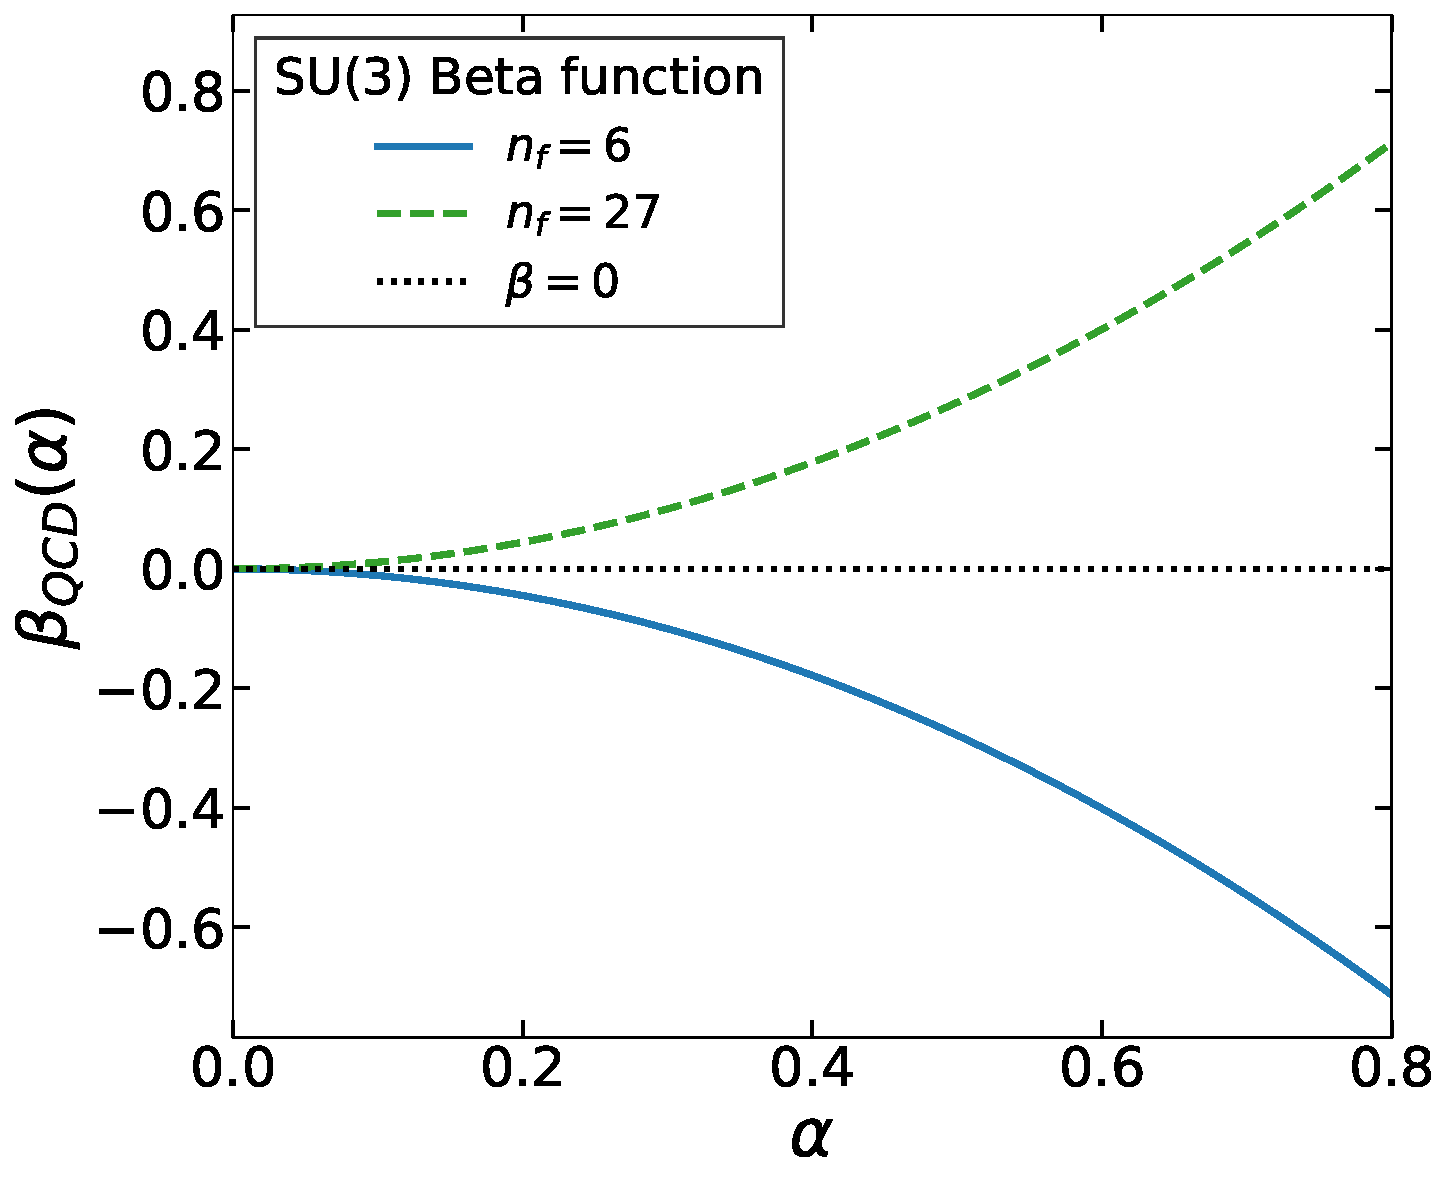
\includegraphics[width=\textwidth]{Figures/beta_function_alpha_pretty.pdf}
       \caption{QCD beta function}
       \label{fig:QCDBeta}
   \end{subfigure}
   \hspace{0.1cm}
   \begin{subfigure}[b]{0.49\textwidth}
       \centering
       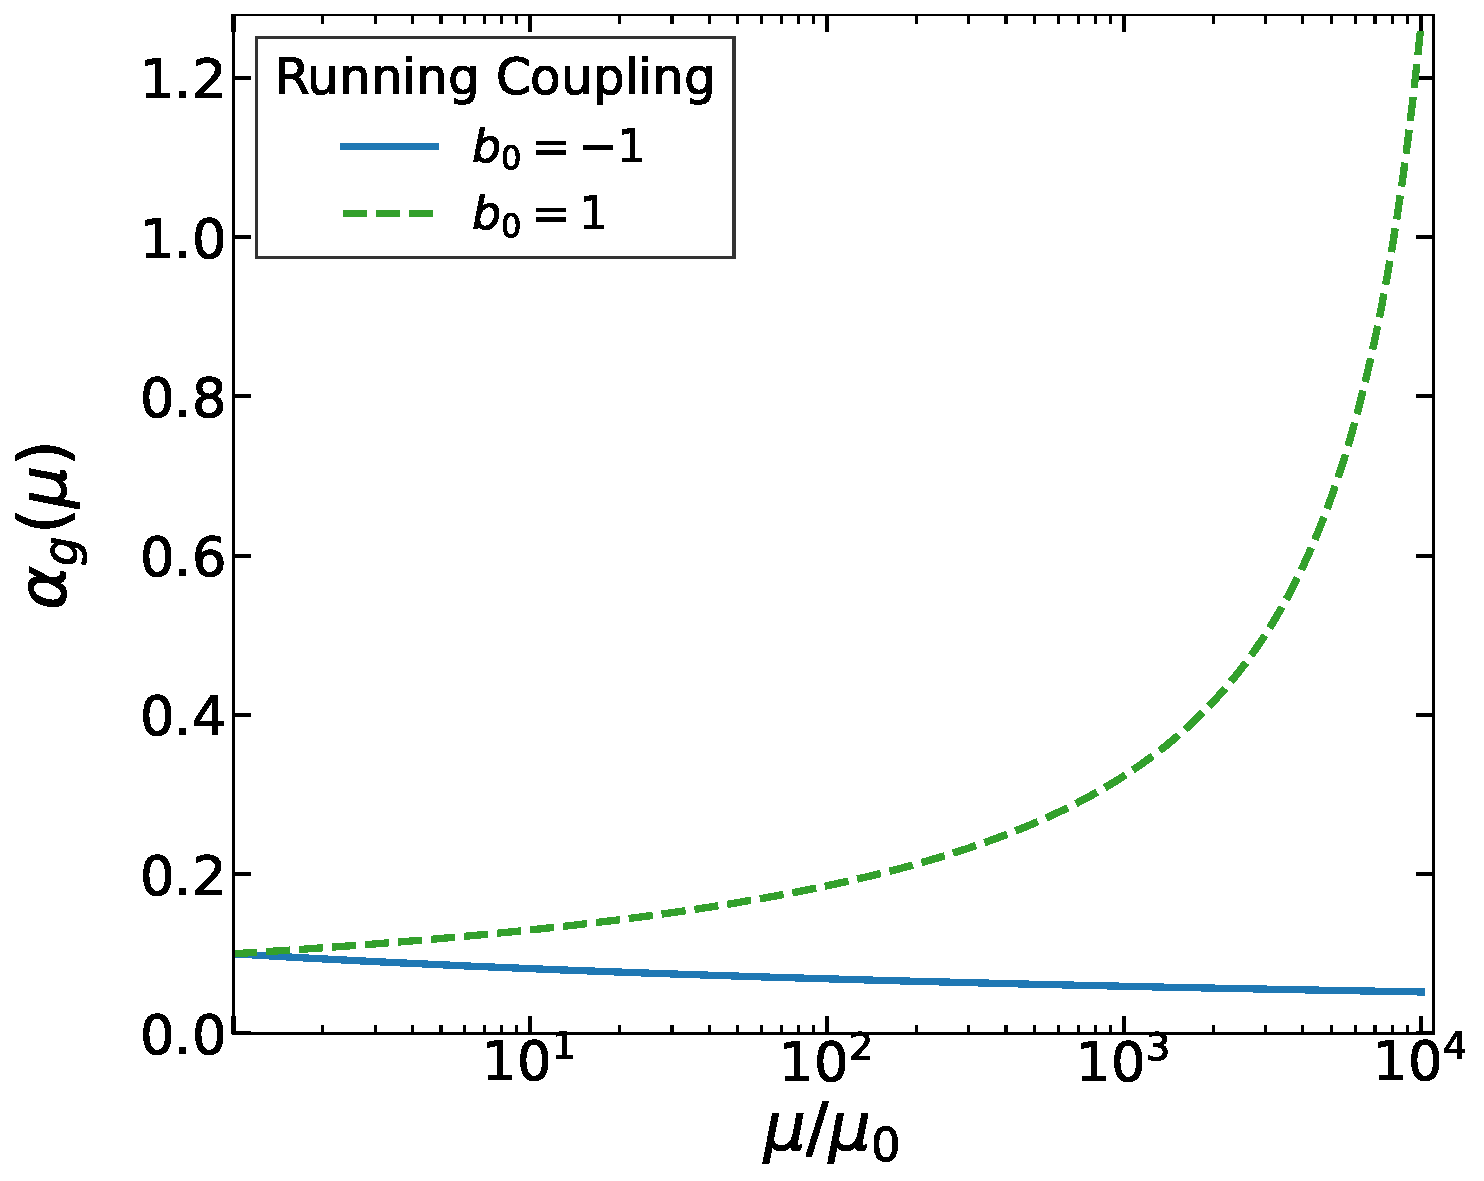
\includegraphics[width=\textwidth]{Figures/running_coupling_pretty-1.pdf}
       \caption{Running of coupling}
       \label{fig:runningcoupling}
   \end{subfigure}
   \caption{The $\SU(3)$ beta function and its corresponding solution. The left panel (A) displays the one-loop beta function for $n_f=6$ (solid blue) and $n_f=27$ (dashed green). The right panel (B) displays the running of the coupling for the two corresponding cases: negative $b_0$ (solid blue) and positive $b_0$ (dashed green).}
   \label{fig:betafunctheory}
\end{figure} 

To understand the dynamical behaviour of our couplings, we must find a solution to the corresponding beta function. We can do this by using separation of variables to solve the RG equation of the gauge coupling. We have the ordinary differential equation  
\begin{align}
    \mu\frac{\dd}{\dd\mu}\alpha_g=b_0\alpha_g^2\,,
\end{align}
where we can separate the variables and integrate
\begin{align}
    \frac{\dd\alpha_g}{\alpha_g^2}=\frac{\dd\ln(\mu)}{\mu}b_0\implies
    \int^{\alpha_g(\mu)}_{\alpha_g(\mu_0)}\frac{\dd\alpha_g}{\alpha_g}=b_0\int^{\mu}_{\mu_0}\frac{\dd\mu}{\mu}\,,
\end{align}
from which we obtain the solution  
\begin{align}
    \alpha_g=\frac{\alpha_{g_0}}{1-b_0 \alpha_{g_0} \ln \left(\frac{\mu}{\mu_0 }\right)}\,,
\end{align}
where $\alpha_{g_0}=\alpha_g(\mu_0)$ and $\mu_0$ is a chosen RG reference scale. The running of the coupling is depicted in Figure~\ref{fig:runningcoupling}, for the two non-trivial scenarios: $b_0>0$ and $b_0<0$. The former case implies a Landau pole at high energies, a characteristic of QED, and matches the fate of the dashed green trajectory in Figure~\ref{fig:QCDBeta}. The latter case demonstrates asymptotically freedom, where the blue solid line converges to zero at high energies, illustrating QCD behaviour.   

It will prove useful in Chapter \ref{chap:GUT} to consider the dependence on $\mu$ of the inverse coupling:
\begin{align}
    \alpha^{-1}_g(\mu)=\frac{1-b_0 \alpha_{g_0} \ln \left(\frac{\mu}{\mu_0 }\right)}{\alpha_{g}(\mu_0)}=\alpha_g^{-1}(\mu_0)-b_0\ln\frac{\mu}{\mu_0}\,.\label{eq:RGinversecoupling}
\end{align}
Now that we have reviewed the renormalisation group, beta functions, and asymptotic freedom, we can move onto discussing the SM and the motivations of GUTs. 